% $Id: conclusion.tex 
% !TEX root = main.tex

%%
\section{Validation}
\label{sec:validation}

This section evaluates \adaptiverl in a realistic traffic‐signal control scenario under non‐stationary congestion. Intelligent traffic management is a canonical application of self‐adaptive systems~\cite{HENRICHS2022106940}, and recent meta‐\ac{RL} work has shown benefits when reward functions change with traffic saturation~\cite{meta-rl-traffic}. Here, we model two crossing lanes (C1 vertical, C2 horizontal) with Poisson arrivals and dynamically switch congestion levels (changing $\lambda$ parameter) to induce concept drift.  

\subsection{Traffic Environment}
We implement a custom \texttt{TrafficEnv} (exending OpenAI's Gym library) whose state is $(c_1,c_2)$, the number of queued vehicles on lanes C1 and C2 (each in $[0,\mathit{max\_state}]$). At each time step the agent selects one of three signal phases:
\[
\{\,(5,2),\;(2,5),\;(3,3)\}
\]
indicating service capacities (percentage of the lane cleared per step) for C1 and C2. During each step, service is applied to C1, new vehicles arrive to C2 (Poisson with rate $\lambda_{2}$), then service is applied to C2, followed by arrivals to C1 (Poisson with rate $\lambda_{1}$). Any unused service capacity incurs a penalty
\[
\mathrm{penalty} \;=\; 3\times(\text{waste}_{C1} + \text{waste}_{C2})\,,
\]
discouraging “over‐serving” when queues are small.

The \emph{dynamic reward} combines congestion cost and service penalty:
\[
r = 
\begin{cases}
-(2c_1 + c_2)\quad &\text{if }c_1>7 \;\wedge\;c_1\ge c_2,\\
-(c_1 + 2c_2)\quad &\text{if }c_2>7 \;\wedge\;c_2>c_1,\\
-(c_1 + c_2)\quad &\text{otherwise}
\end{cases}
\;-\;\mathrm{penalty}\,.
\]
Episodes last 30 steps. We induce two concept drifts by changing arrival rates at episodes 3,000 and 8,000:
\[
(\lambda_1,\lambda_2):
\;(4,2)\;\to\;(5,7)\;\to\;(3,1).
\]

We compare:
\begin{itemize}
  \item A \emph{standard Q‐learning} agent with fixed $\alpha=0.1$, $\gamma=0.9$, and $\varepsilon$ decayed exponentially to $0.01$.
  \item An \emph{\adaptiverl} agent that uses the PH‐test to detect drifts in episode‐rewards, resets $\varepsilon\!=\!1$ upon detection, and adaptively adjusts $\alpha$ based on the TD‐error (cf.\ Section~\ref{sec:implementation}).  When a drift is detected, it also \emph{appends} two new phases
  \[
    (7,3)\quad\text{and}\quad(3,7),
  \]
  allowing finer control under high congestion. Old actions are never removed.
\end{itemize}

\subsection{Results}
Figure~\ref{fig:traffic-learning-curve} plots the cumulative mean reward (over the last 500 episodes) for both agents. The green vertical line marks the PH‐test detection at episode 3004; the second drift at episode 8000 was not flagged, since the new arrival rates produce a reward distribution within the original sensitivity threshold.

\begin{figure*}
    \centering
    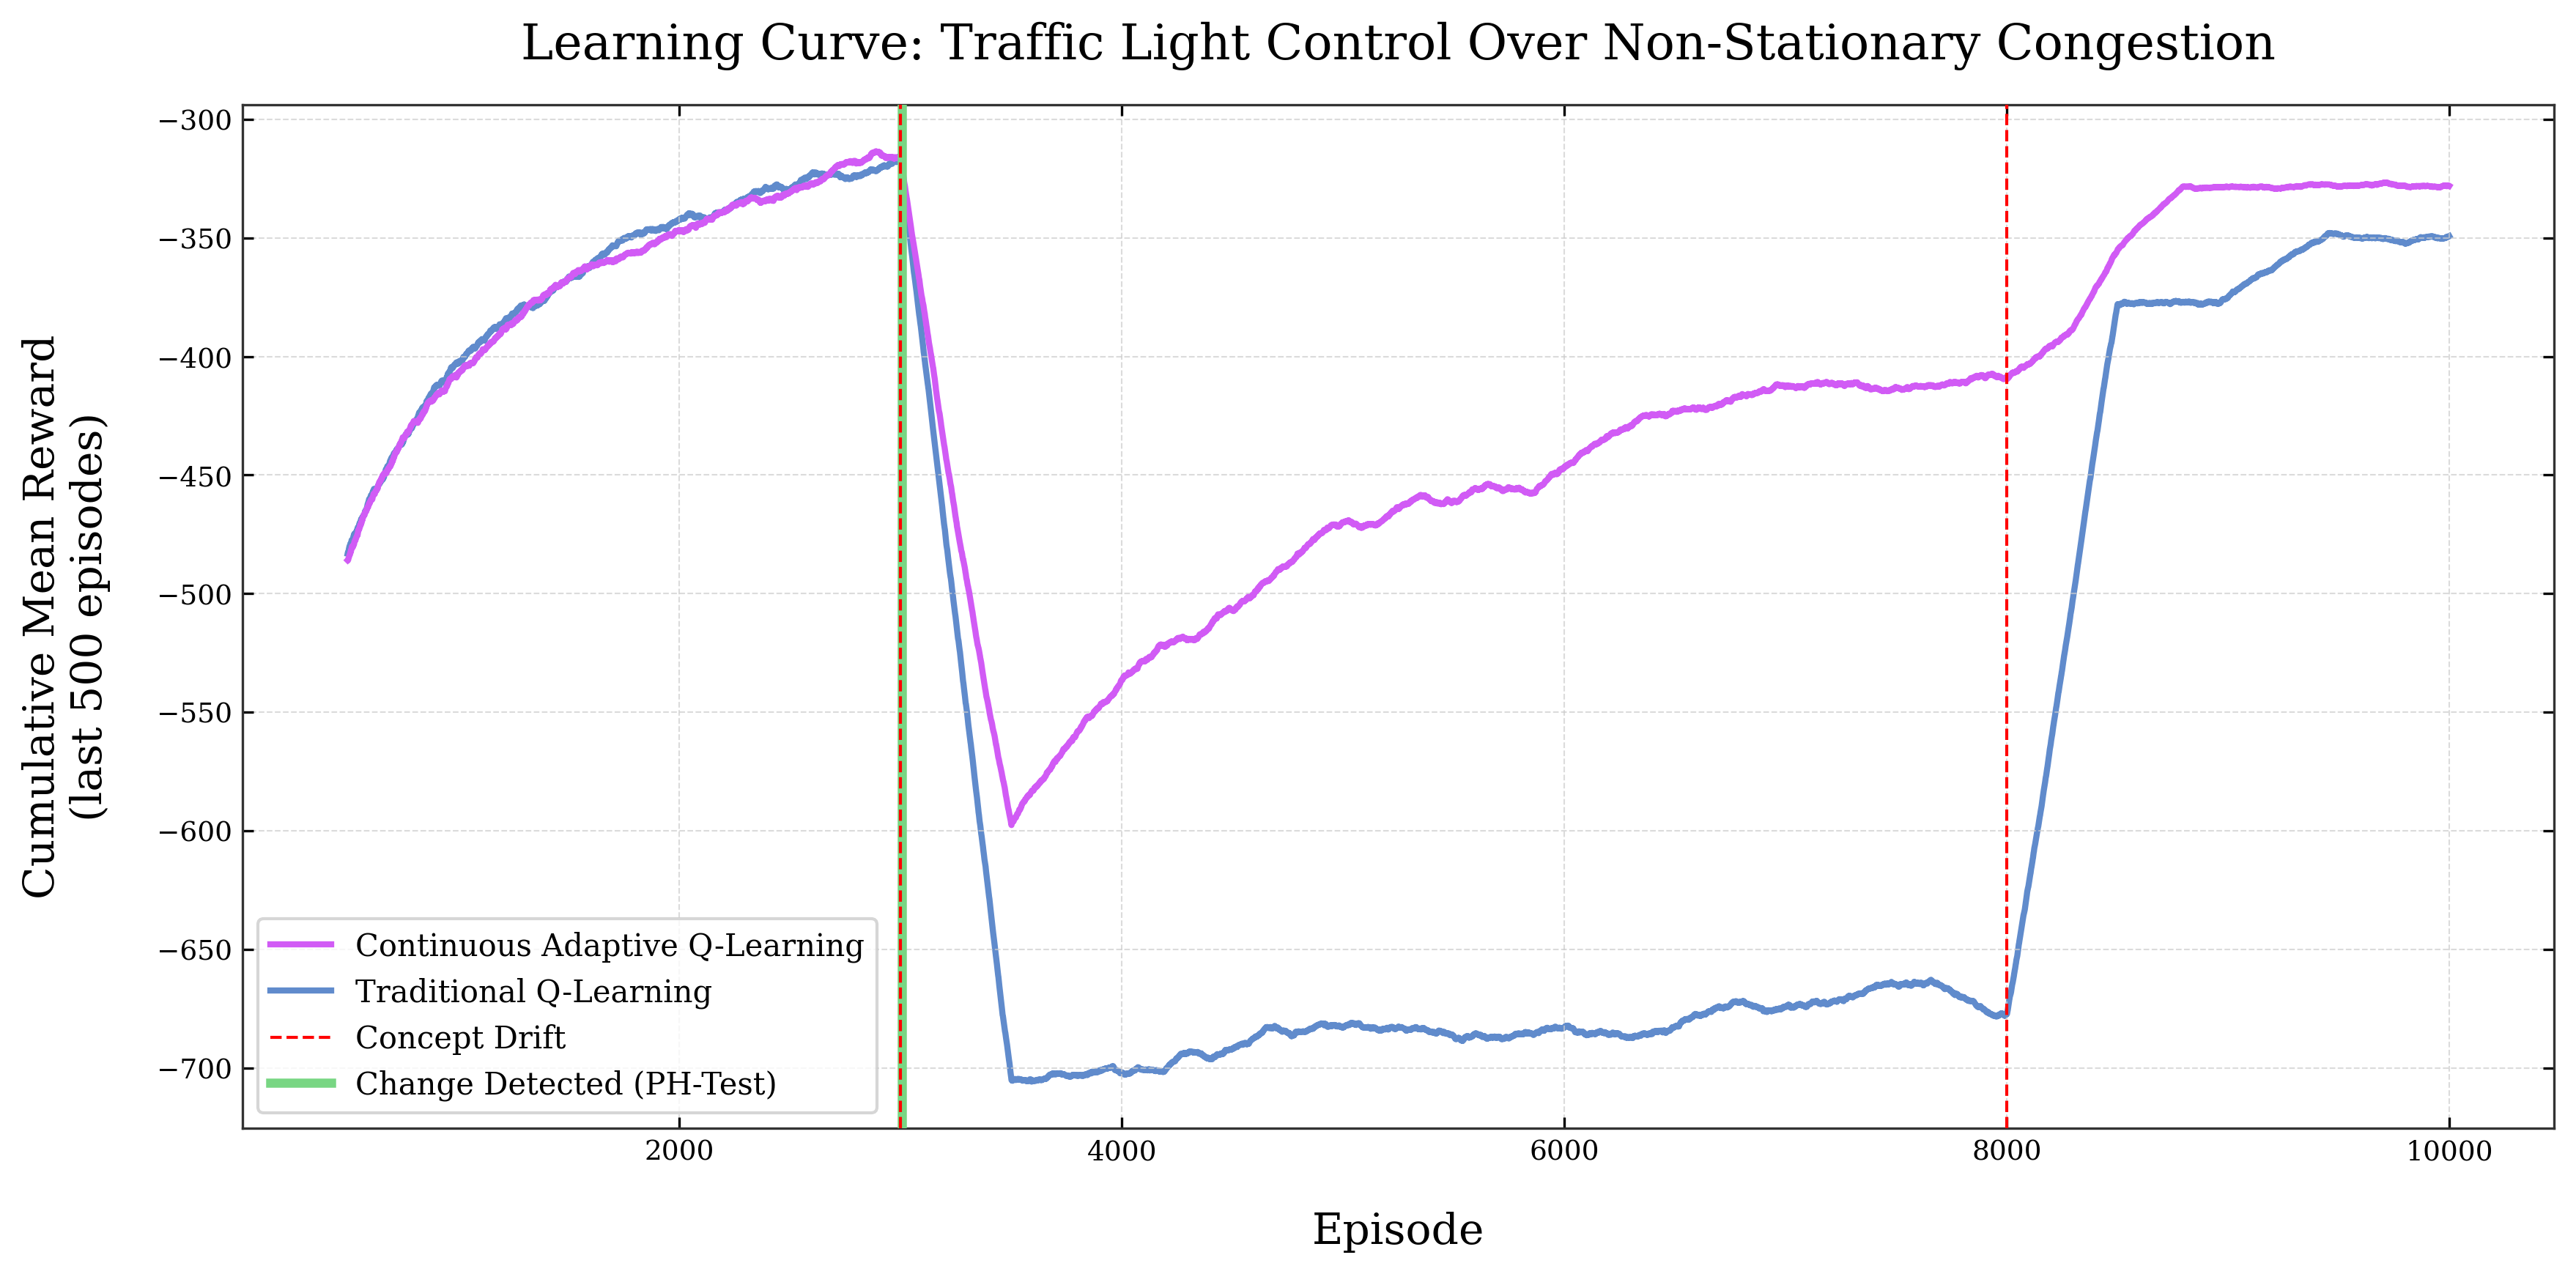
\includegraphics[width=\textwidth]{figures/traffic_learning_curve.png}
    \caption{Learning curves for traffic‐signal control under non‐stationary congestion. Rapidly recovers after the first drift thanks to extension of action set after PH-Test detection, while traditional Q-learning suffers prolonged performance drops.}
    \label{fig:traffic-learning-curve}
\end{figure*}

Initially, both agents improve steadily. After the first drift, \adaptiverl promptly increases exploration, exploits its new actions $(7,3)$ and $(3,7)$, and regains performance within a few hundred episodes. In contrast, the standard agent endures a deep, slow recovery. The built-in penalty for wasted green time ensures \adaptiverl does not “over‐serve” when queues shrink, automatically balancing old and new phases without discarding any actions.

Quantitatively, over 10 000 episodes:
\begin{itemize}
  \item \adaptiverl achieves a higher average reward (–415 vs.\ –530) and a smaller worst‐case drop (-770 vs.\ –792).
  \item add more
\end{itemize}

This traffic‐signal case confirms that \adaptiverl can:
\begin{enumerate}
  \item Detect and react to non-stationary congestion via the PH-test, boosting exploration exactly when needed and the adaptive mechanisms that distinguish \adaptiverl.
  \item Seamlessly incorporate new signal phases—analogous to real‐world reprogramming of traffic lights—without removing prior options.
  \item Leverage a dynamic reward (with penalization) to avoid excessive service when traffic is light, resulting in resource‐efficient policies.
\end{enumerate}
In practice, modern traffic controllers can update phase timings in real time; endowing them with self-adaptive intelligence, as in \adaptiverl, allows continuous, automated adjustment to changing traffic patterns without manual retuning.

\endinput

